% aspect ratio: 16:9
\documentclass[unicode, 9pt, aspectratio=169]{beamer}
\usepackage{mybeamer}

% uncomment the following lines when you use tikz
%\usepackage{tikz}
%\usetikzlibrary{positioning, calc, arrows.meta}

%%%%%%%%%%%%%%%%%%%%%%%%%
% note
%%%%%%%%%%%%%%%%%%%%%%%%%
% you can write notes on your presentation here.
% e.g. how much time you spend in each page

%%%%%%%%%%%%%%%%%%%%%%%%%
% document
%%%%%%%%%%%%%%%%%%%%%%%%%
% title
\title{beamerでスライドをつくるときのtipsなど}
\author{妙寺 菜麻江 (MYOJI Namae)}
\institute{所属,institute}
\date{\today}

% main
\begin{document}
%\pagenumbering{arabic} % uncomment if you use romannum package: or page numbers would be in roman numbers

\maketitle

% main text
\begin{frame}[containsverbatim] % beamer and verb / verbatim are incompatible in default
\frametitle{main.texとmybeamer.styについて}
このテーマはmetropolisをベースに,mybeamer.styの中でカスタマイズしたものです.

main.texのプリアンブルで\verb+\usepackage{mybeamer}+としてmybeamer.styを読み込んでいます.

\begin{block}{}
\begin{itemize}
    \item sectionを指定すると,section titleページが挿入される.
    \item ページ数は,右下に「このページ / 全体」の形で表示される.
    \item 各ページの下にはプログレスバー(オレンジとグレー)が表示されている.
    \item emphコマンドは\emph{太字}になるように上書きしてある.
\end{itemize}
\end{block}
\end{frame}

\section{ここがsection title ページ}

\begin{frame}[label=block page] % 再掲するために名前をつける
\frametitle{block環境を例示する}
3種類のblock環境があり,一部に手を入れてある.
\begin{block}{普通のblock}
    角丸,影なし.
\end{block}

\begin{alertblock}{これはalertblock}
    色を調整した.
\end{alertblock}

\begin{exampleblock}{exampleblockは緑色}
    exampleblockには特に調整をしていない.
\end{exampleblock}

*このスライドにはblock pageというラベルを与えてあり,あとで呼び出して再掲できる,
\end{frame}

\section{スライドを水平方向に分割したい}

\begin{frame}
\frametitle{左右に分割したいときはcolumns環境を使うのが便利}
\centering

\begin{block}{このページを水平方向に,3面に分割する}
\begin{itemize}
    \item 左からlinewidthの20\%,30\%,40\%(合計90\%)に分割する.
    \item clolumn間の余白を考慮すると,columnの幅の合計はlinewidth(100\%)よりも小さい方が無難.
\end{itemize}
\end{block}
\vspace{\baselineskip}

\begin{columns}
    \begin{column}{.2\linewidth}
        linewidthの20\%の幅

        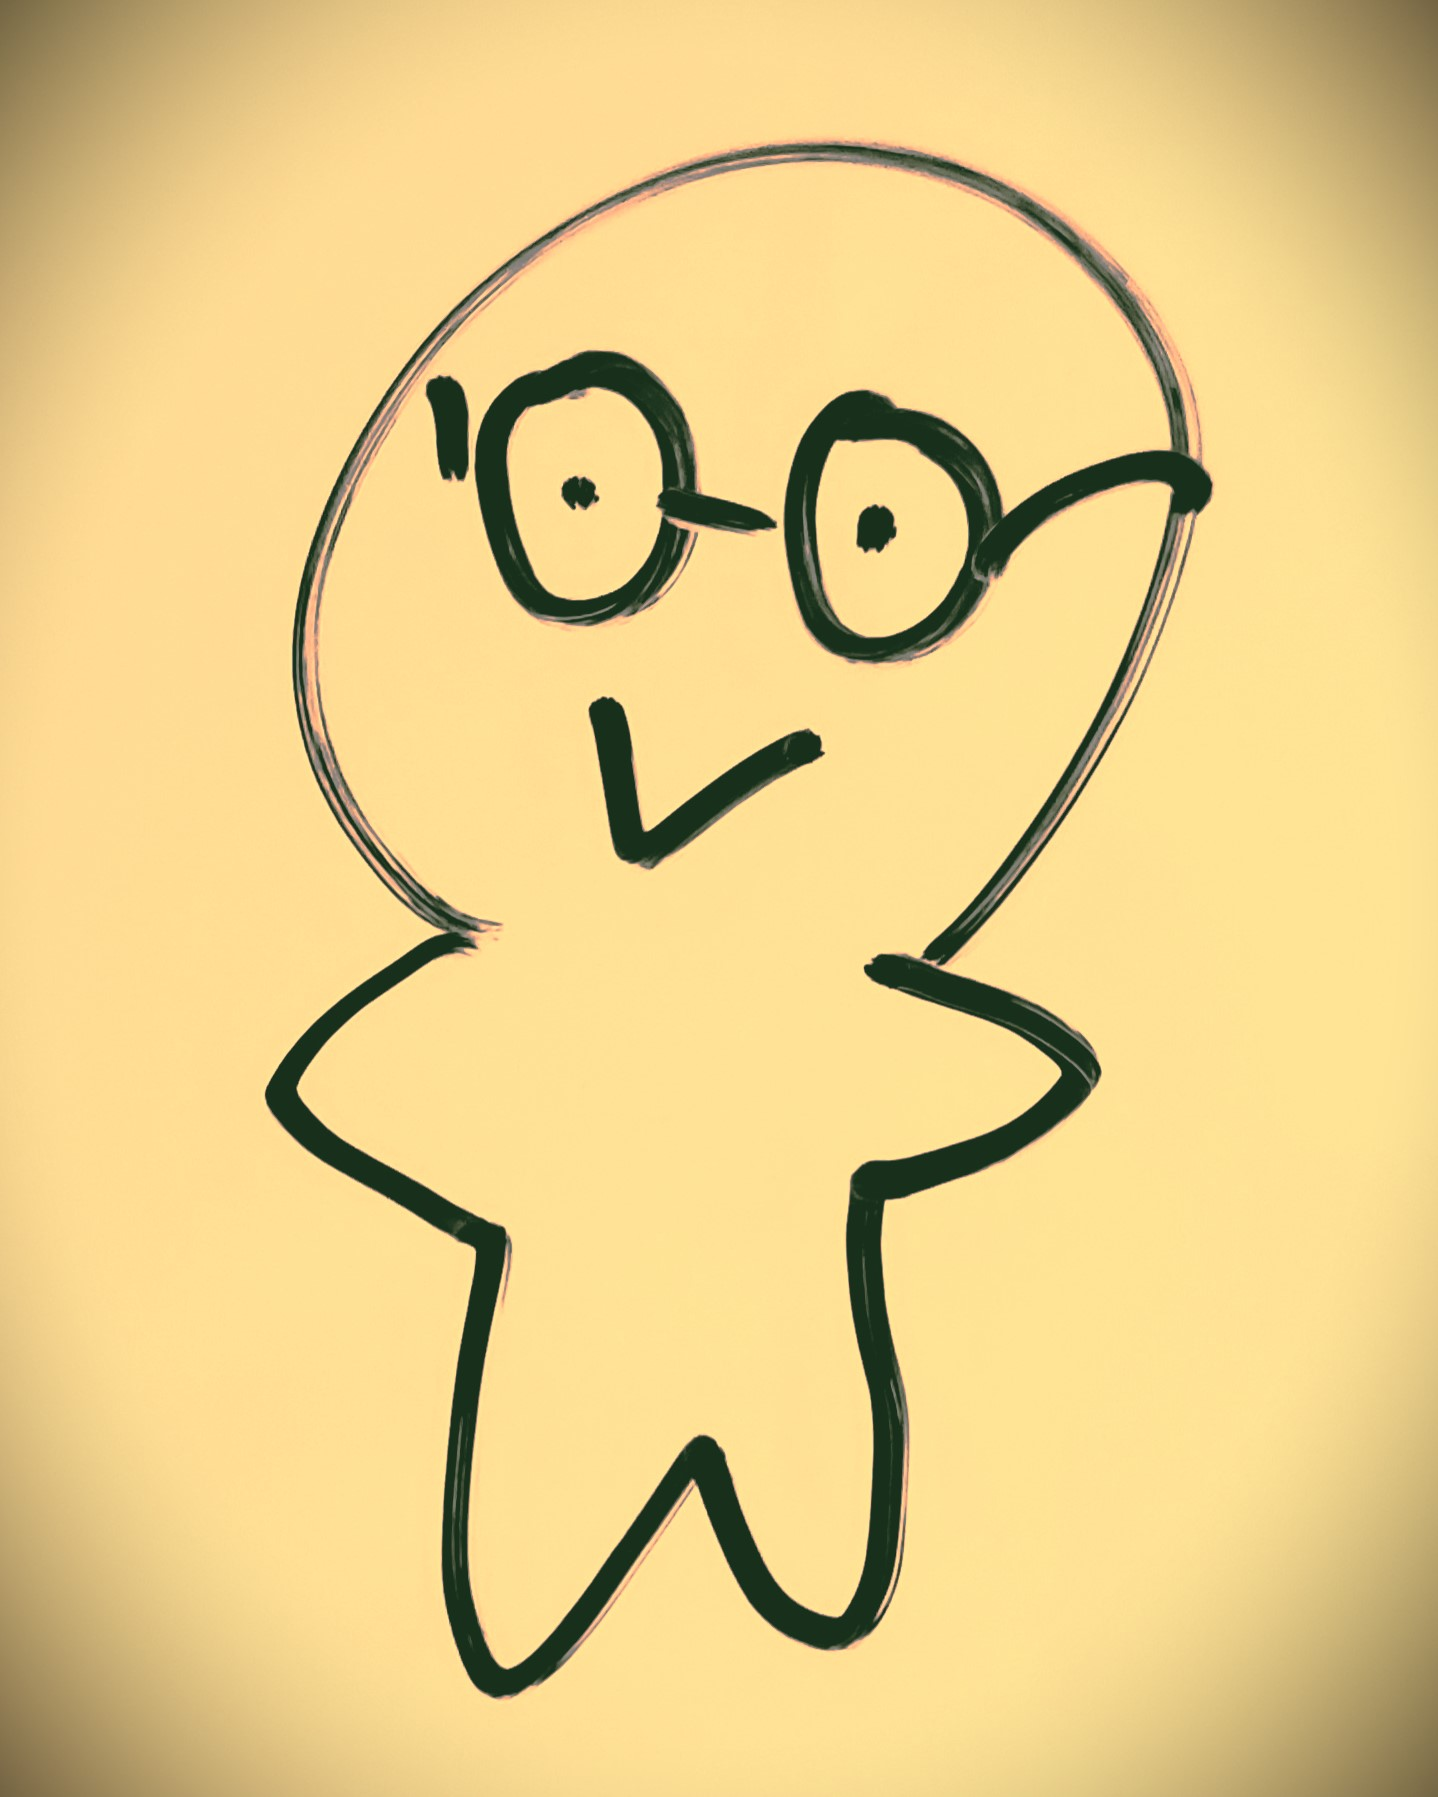
\includegraphics[height=.25\textheight, width=\linewidth]{figs/fig_mod.jpg}
    \end{column}
    \begin{column}{.3\linewidth}
        \centering
        \hrulefill

        \begin{itemize}
            \item 幅いっぱいの罫線をひいた.
            \item hrulefillを使った.
        \end{itemize} 
    \end{column}
    %\hspace{5pt}
    \vrule \hspace{5pt}
    \begin{column}{.4\linewidth}
        \hrulefill

        この例ではcolumn幅の合計がlinewidthの90\%である(100\%ではない).
    \end{column}
\end{columns}
\vspace{10pt}

\begin{minipage}{.7\linewidth}
    \begin{roundbox}{\linewidth}
    \centering
    上の例では2つ目と3つ目のcolumn環境の間に

    \backslash vrule \backslash hspace \{5pt\}

    と書き,区切り線を入れた.
    \end{roundbox}
\end{minipage}
\end{frame}

\begin{frame}
\frametitle{ページを左右に分割する別の方法もある}
でも,\emph{結局columnsを使うのが楽で安定している}ように思う.

\begin{center}
このcenter環境の中に,\emph{minipage}を2つ配置しよう.
\vspace{-8pt}

\hrulefill

\begin{minipage}{.4\linewidth}
    \begin{itemize}
        \item 愚直にminipageを並べれば,左右に分割される.
        \item ここでは40\%のminipageを2つ配置している.
        \item 幅の合計がlinewidthを超えないように注意!
    \end{itemize}
\end{minipage}
%
\hspace{12pt}
%
\begin{minipage}{.4\linewidth}
\begin{itemize}
    \item こういうときに配置がおかしくなる:
    \begin{itemize}
        \item minipageの幅の和が大きすぎた
        \item minipage環境の直前・直後に改行した
    \end{itemize}
    \item 左右が近すぎるので,minipageの間にhspaceをいれている.
    \item[$\to$] 調整することが多い!
\end{itemize}
\end{minipage}
\end{center}

\hrulefill
\begin{center}
    \emph{tabular}環境を使うと挙動は安定する.
    \vspace{-8pt}

    \hrulefill

    \begin{tabular}{cc}
        \begin{minipage}{.5\linewidth}
            tabular環境の中にminipage環境を並べればよい.
            \begin{block}{}
                \centering
                普通の文書で図を並べたいときにも使える.
            \end{block}
        \end{minipage}
        &
        \begin{minipage}{.4\linewidth}
            \begin{itemize}
                \item ここは右の行です.
                \item 改行されてしまう問題を回避できる.
                \item でもコードが煩雑になる印象.
            \end{itemize}
        \end{minipage}
    \end{tabular}
\end{center}
\end{frame}

\section{ページ内の要素の幅を調節したい}
\begin{frame}
\frametitle{minipageを使ってblockなどの幅を調整する(1)}
ある要素がスライドの幅いっぱいに拡がってほしいわけではない,という場面がよくある.
\begin{block}{}
    \centering
    block環境は幅を指定できない.もっと狭くていいのに.
\end{block}

\hrulefill
\begin{center}
center環境の上下に罫線を引きました.
\begin{itemize}
    \item 例えばitemizeは長い項目がなくても,ページの幅いっぱいに
    \item スペースをとるから,左寄りに配置されて変な感じになる.
    \item 中央揃えしたくてcenter(ing)を使うのに!
\end{itemize}
\end{center}
\hrulefill
\end{frame}

\begin{frame}
\frametitle{minipageを使ってblockなどの幅を調整する(2)}
\centering
\begin{block}{}
    \centering
    普通にblock環境をつくると,ページ幅いっぱいになってしまう.
\end{block}

\begin{minipage}{.8\linewidth}
    \begin{alertblock}{center(ing)とminipage環境を組み合わせるとよい!}
    \centering
    block環境はminipage環境の幅いっぱいに配置される.

    ここでは,minipage環境の中にalertblockを配置した.
    \end{alertblock}

    \begin{itemize}
        \item itemizeの位置も変わるので,調整次第で中央揃え感も出せる.
        \item[*] itemizeをずらすだけならhspaceを使ってもよい.
    \end{itemize}
\end{minipage}

キーワードだけ強調したいときなどは,もっと狭くてもいいだろう.
\begin{minipage}{.5\linewidth}
    \begin{exampleblock}{}
        \centering
        \Large \emph{キーワード}
    \end{exampleblock}
\end{minipage}
\end{frame}

\section{frameに名前をつけて,あとで再掲することもできる}
\againframe{block page} % 1ページ目を再掲する

\section{図を並べて配置したい}
\begin{frame}
\frametitle{tabular環境を使うと安定して図を並べられる(1)}
図を水平方向に並べる場合,includegraphicsのoptionに幅(width)ではなく高さ(height)を指定する方が見た目を整えやすい.

\begin{center}
    \begin{minipage}{.7\linewidth}
        \begin{block}{}
            \centering
            \begin{tabular}{ccc}
                1列目 & 2列目 & 3列目 \\ \midrule
                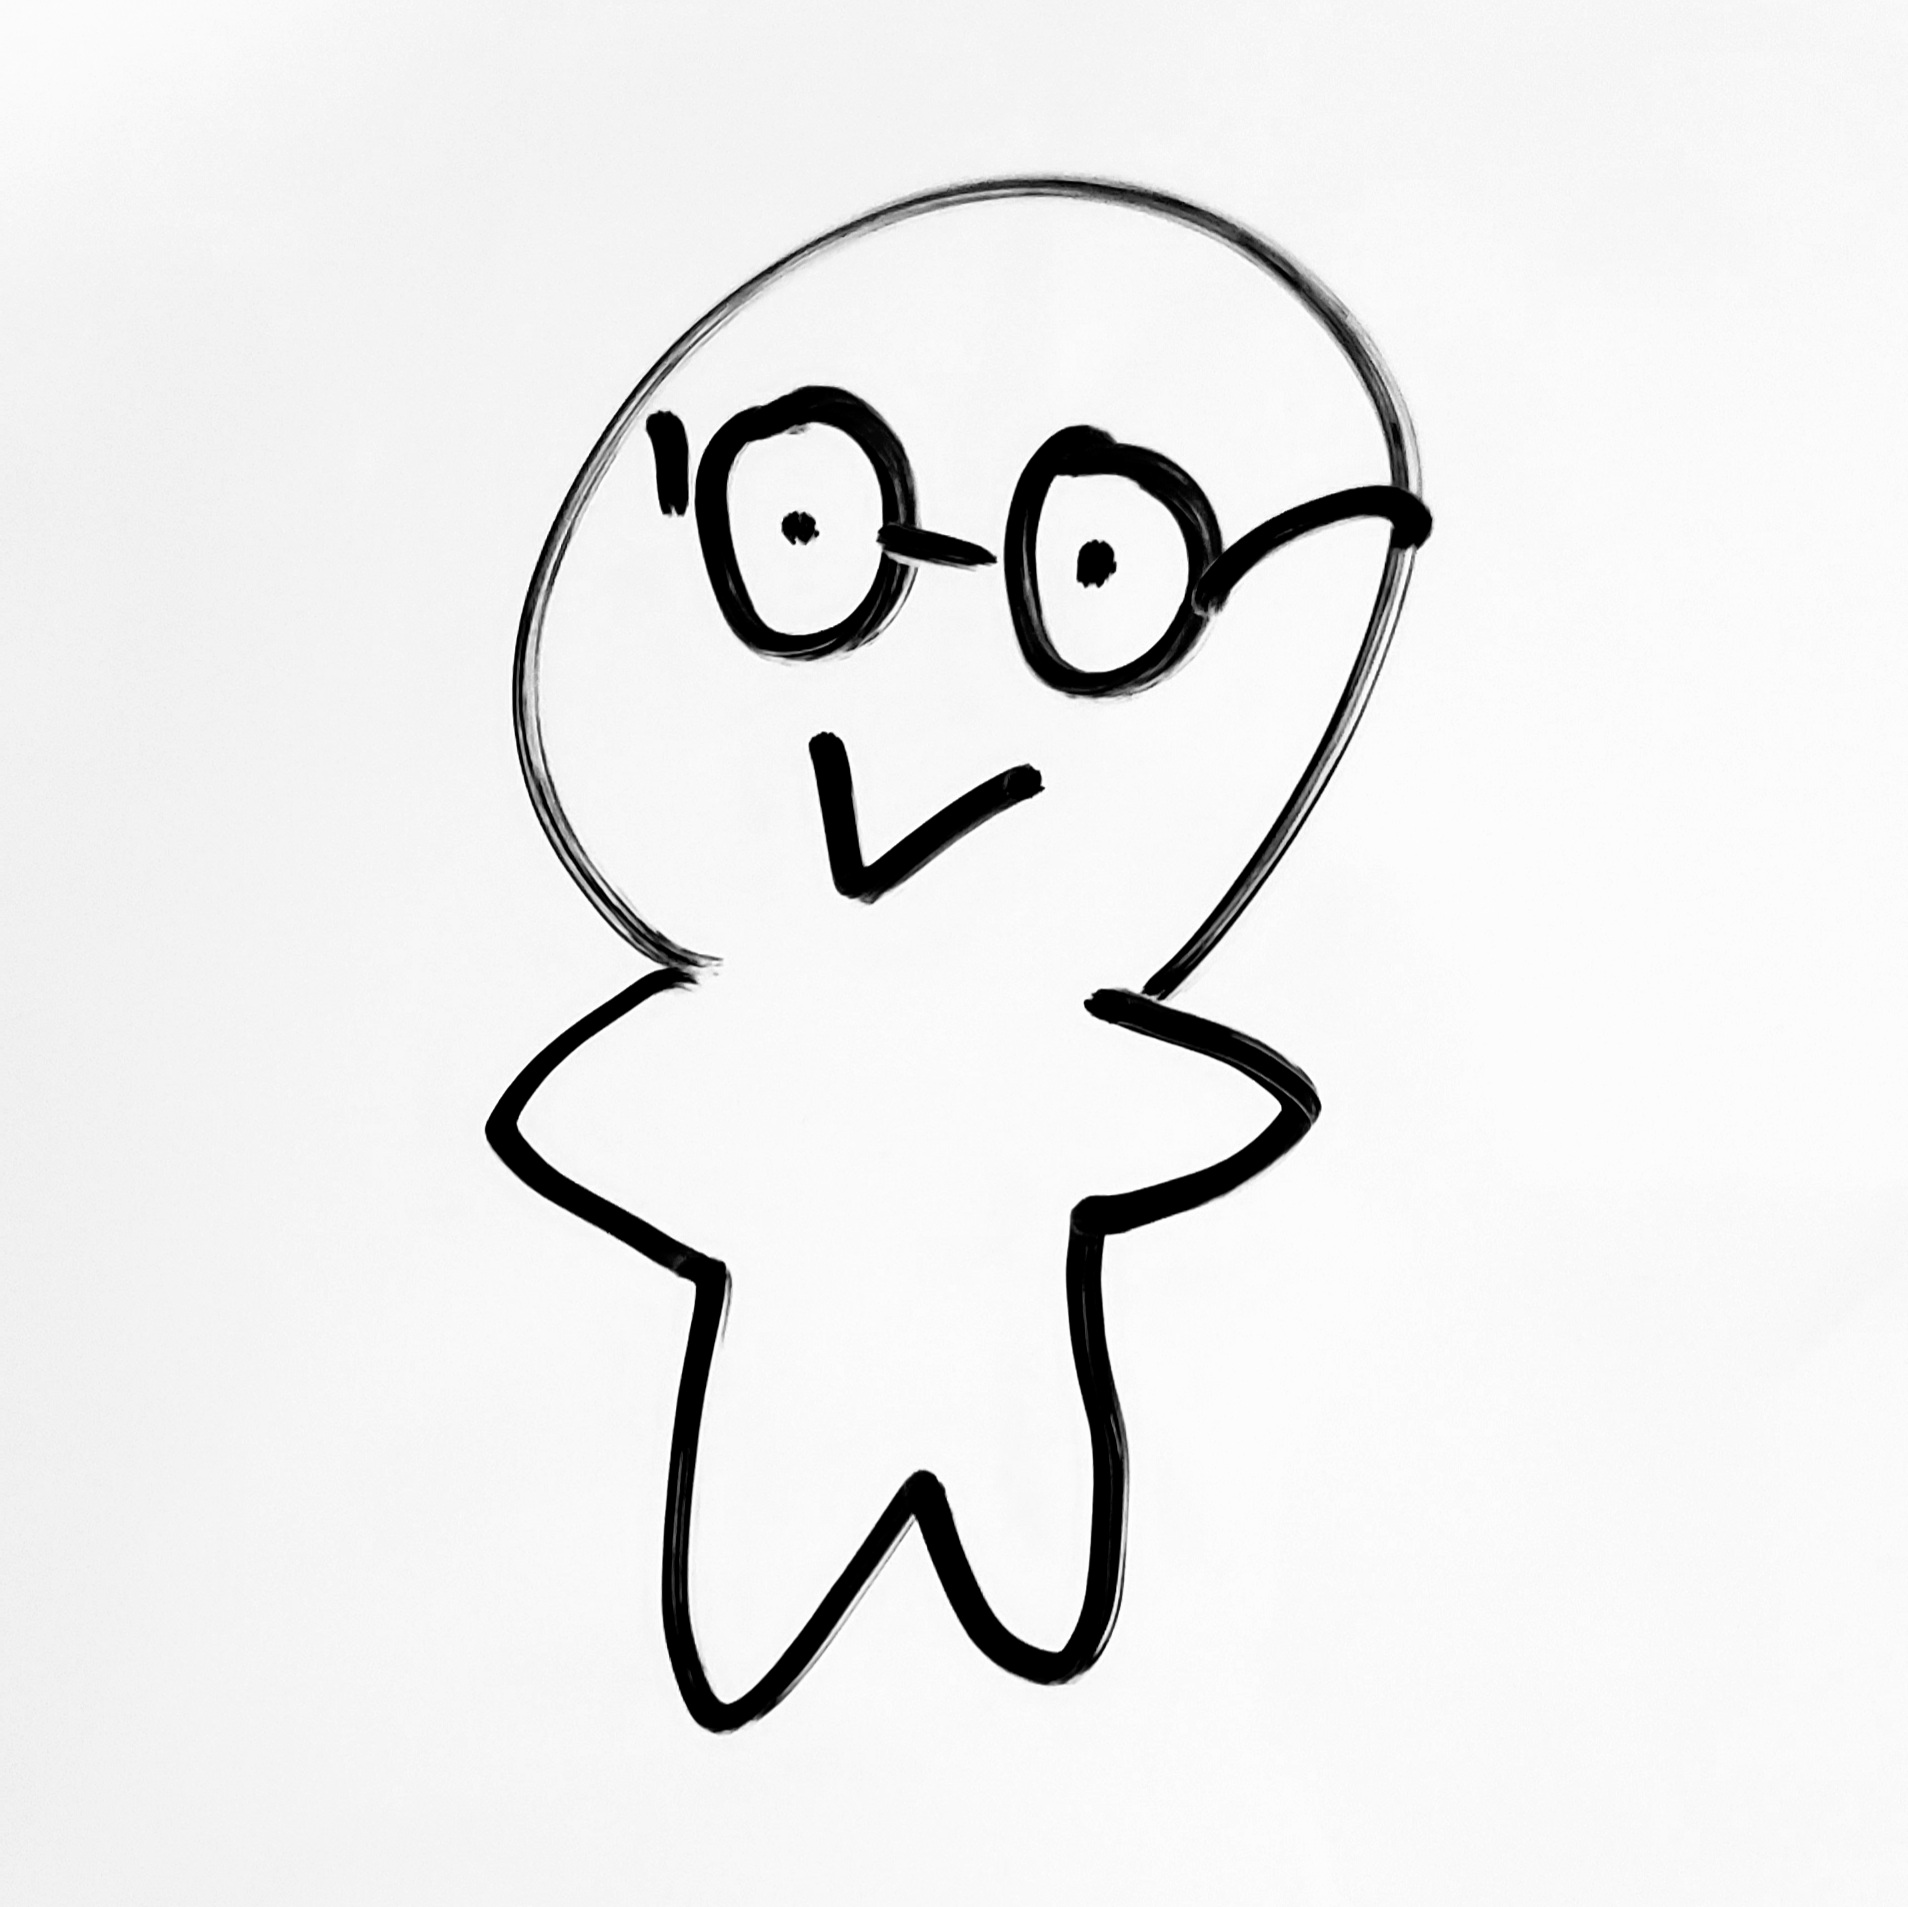
\includegraphics[height=.3\textheight]{figs/fig.jpg}
                &
                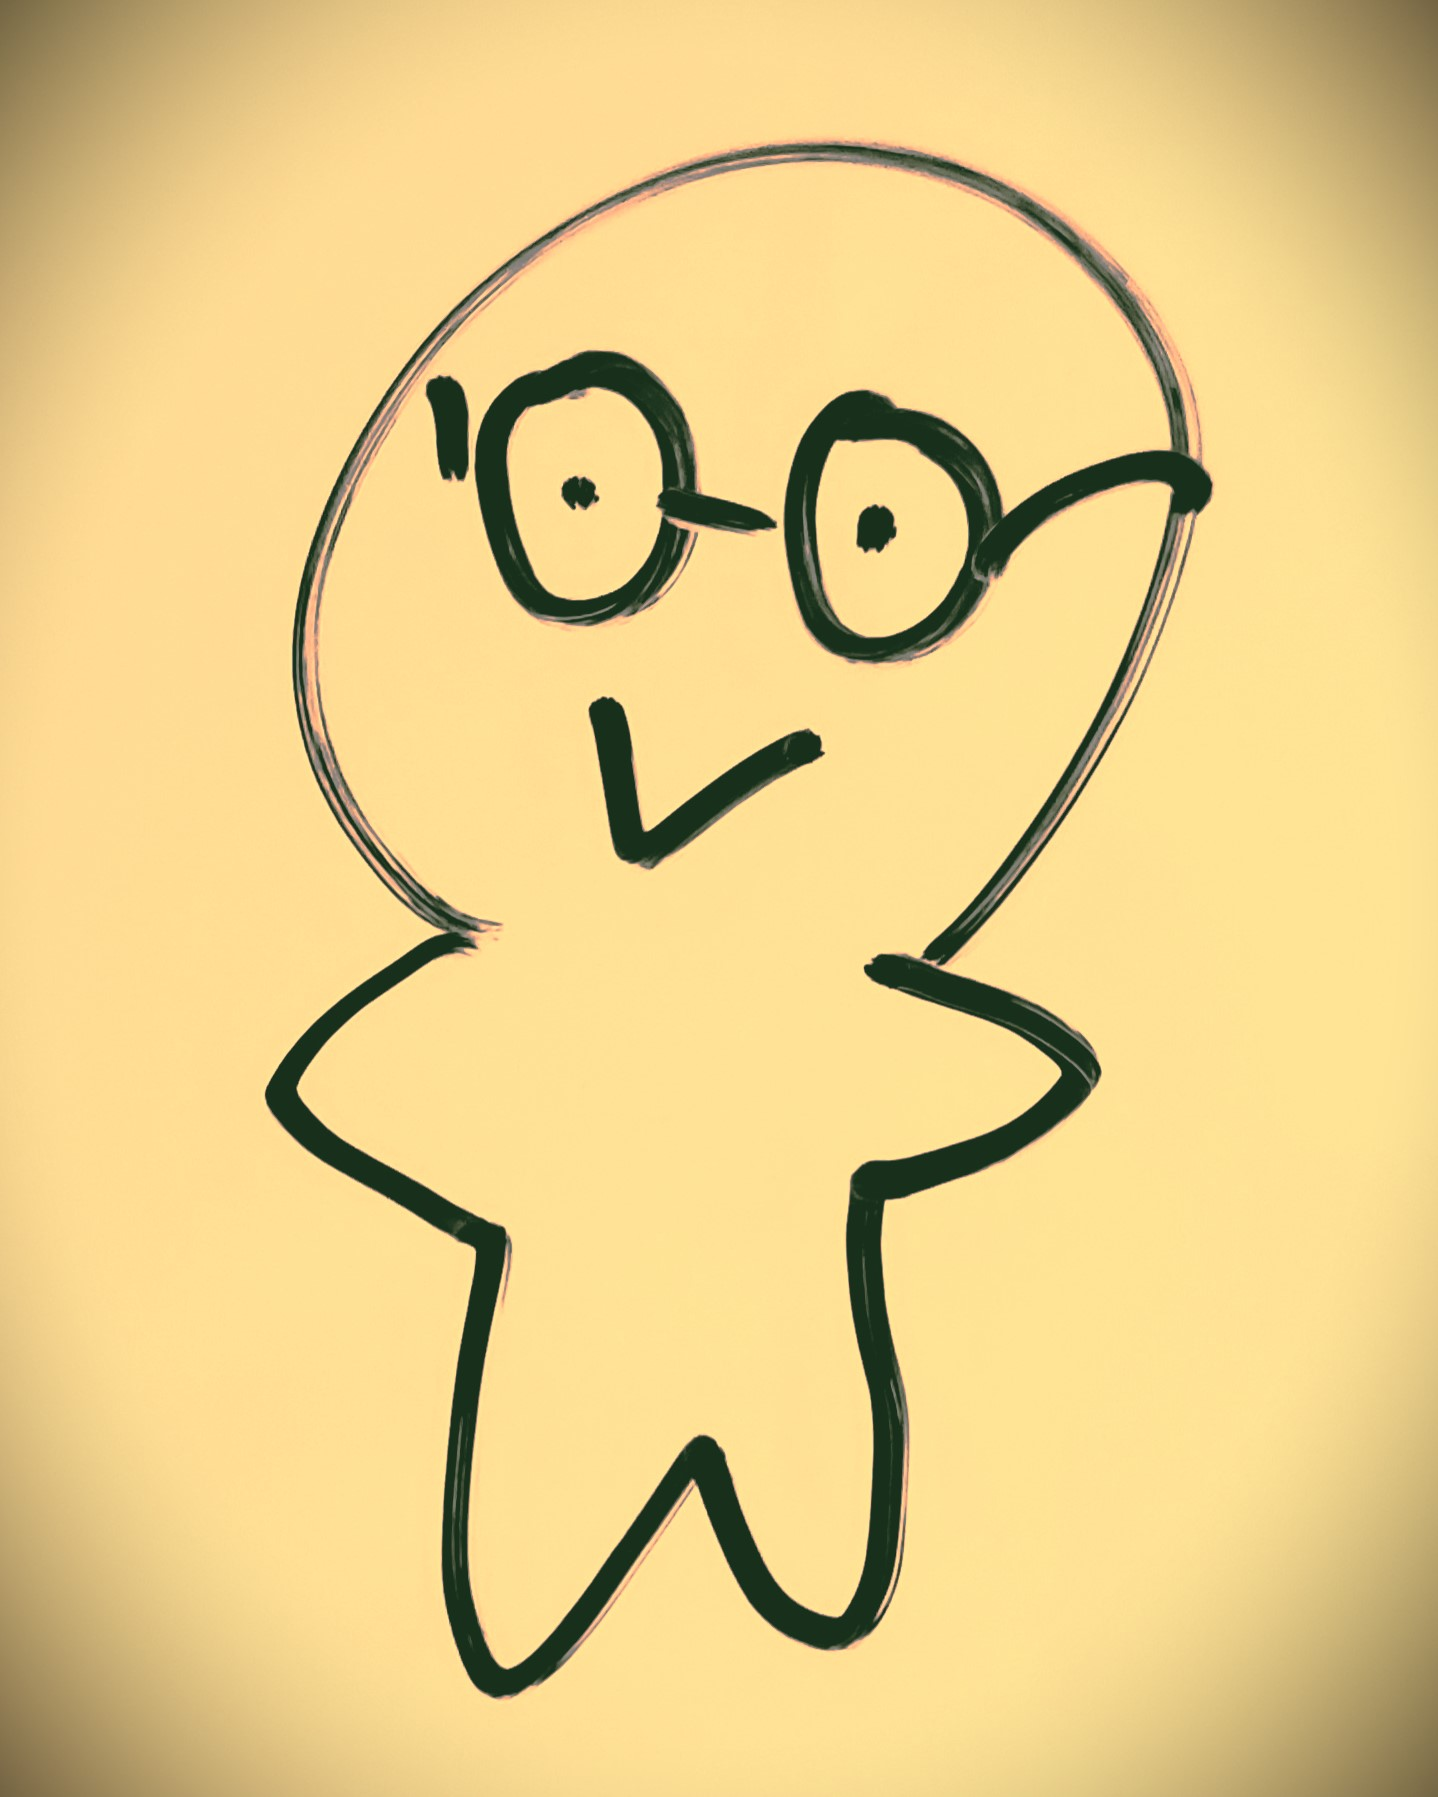
\includegraphics[height=.3\textheight]{figs/fig_mod.jpg}
                &
                \makecell{makecellを使うと \\ セル内で改行もできる}
            \end{tabular}
        \end{block}
    \end{minipage}
\end{center}

$\to$ tabular環境内にそのままincludegraphicsとテキスト等を置くと,垂直方向の配置が合わない.
\end{frame}

\begin{frame}[containsverbatim]
\frametitle{tabular環境を使うと安定して図を並べられる(2)}
$\blacksquare$ tabular環境内にそのままincludegraphicsとテキスト等を置くと,垂直方向の配置が合わない.
\begin{itemize}
    \item これはincludegraphicsのベースラインが図の下端に設定されるため,らしい.
    \item raiseboxコマンドで垂直方向に位置を調整すれば解決する.
\end{itemize}

\begin{center}
\begin{minipage}{.7\linewidth}
\begin{block}{}
\centering
\begin{tabular}{ccc}
    1列目 & 2列目 & 3列目 \\ \midrule
    \raisebox{-.5\height}{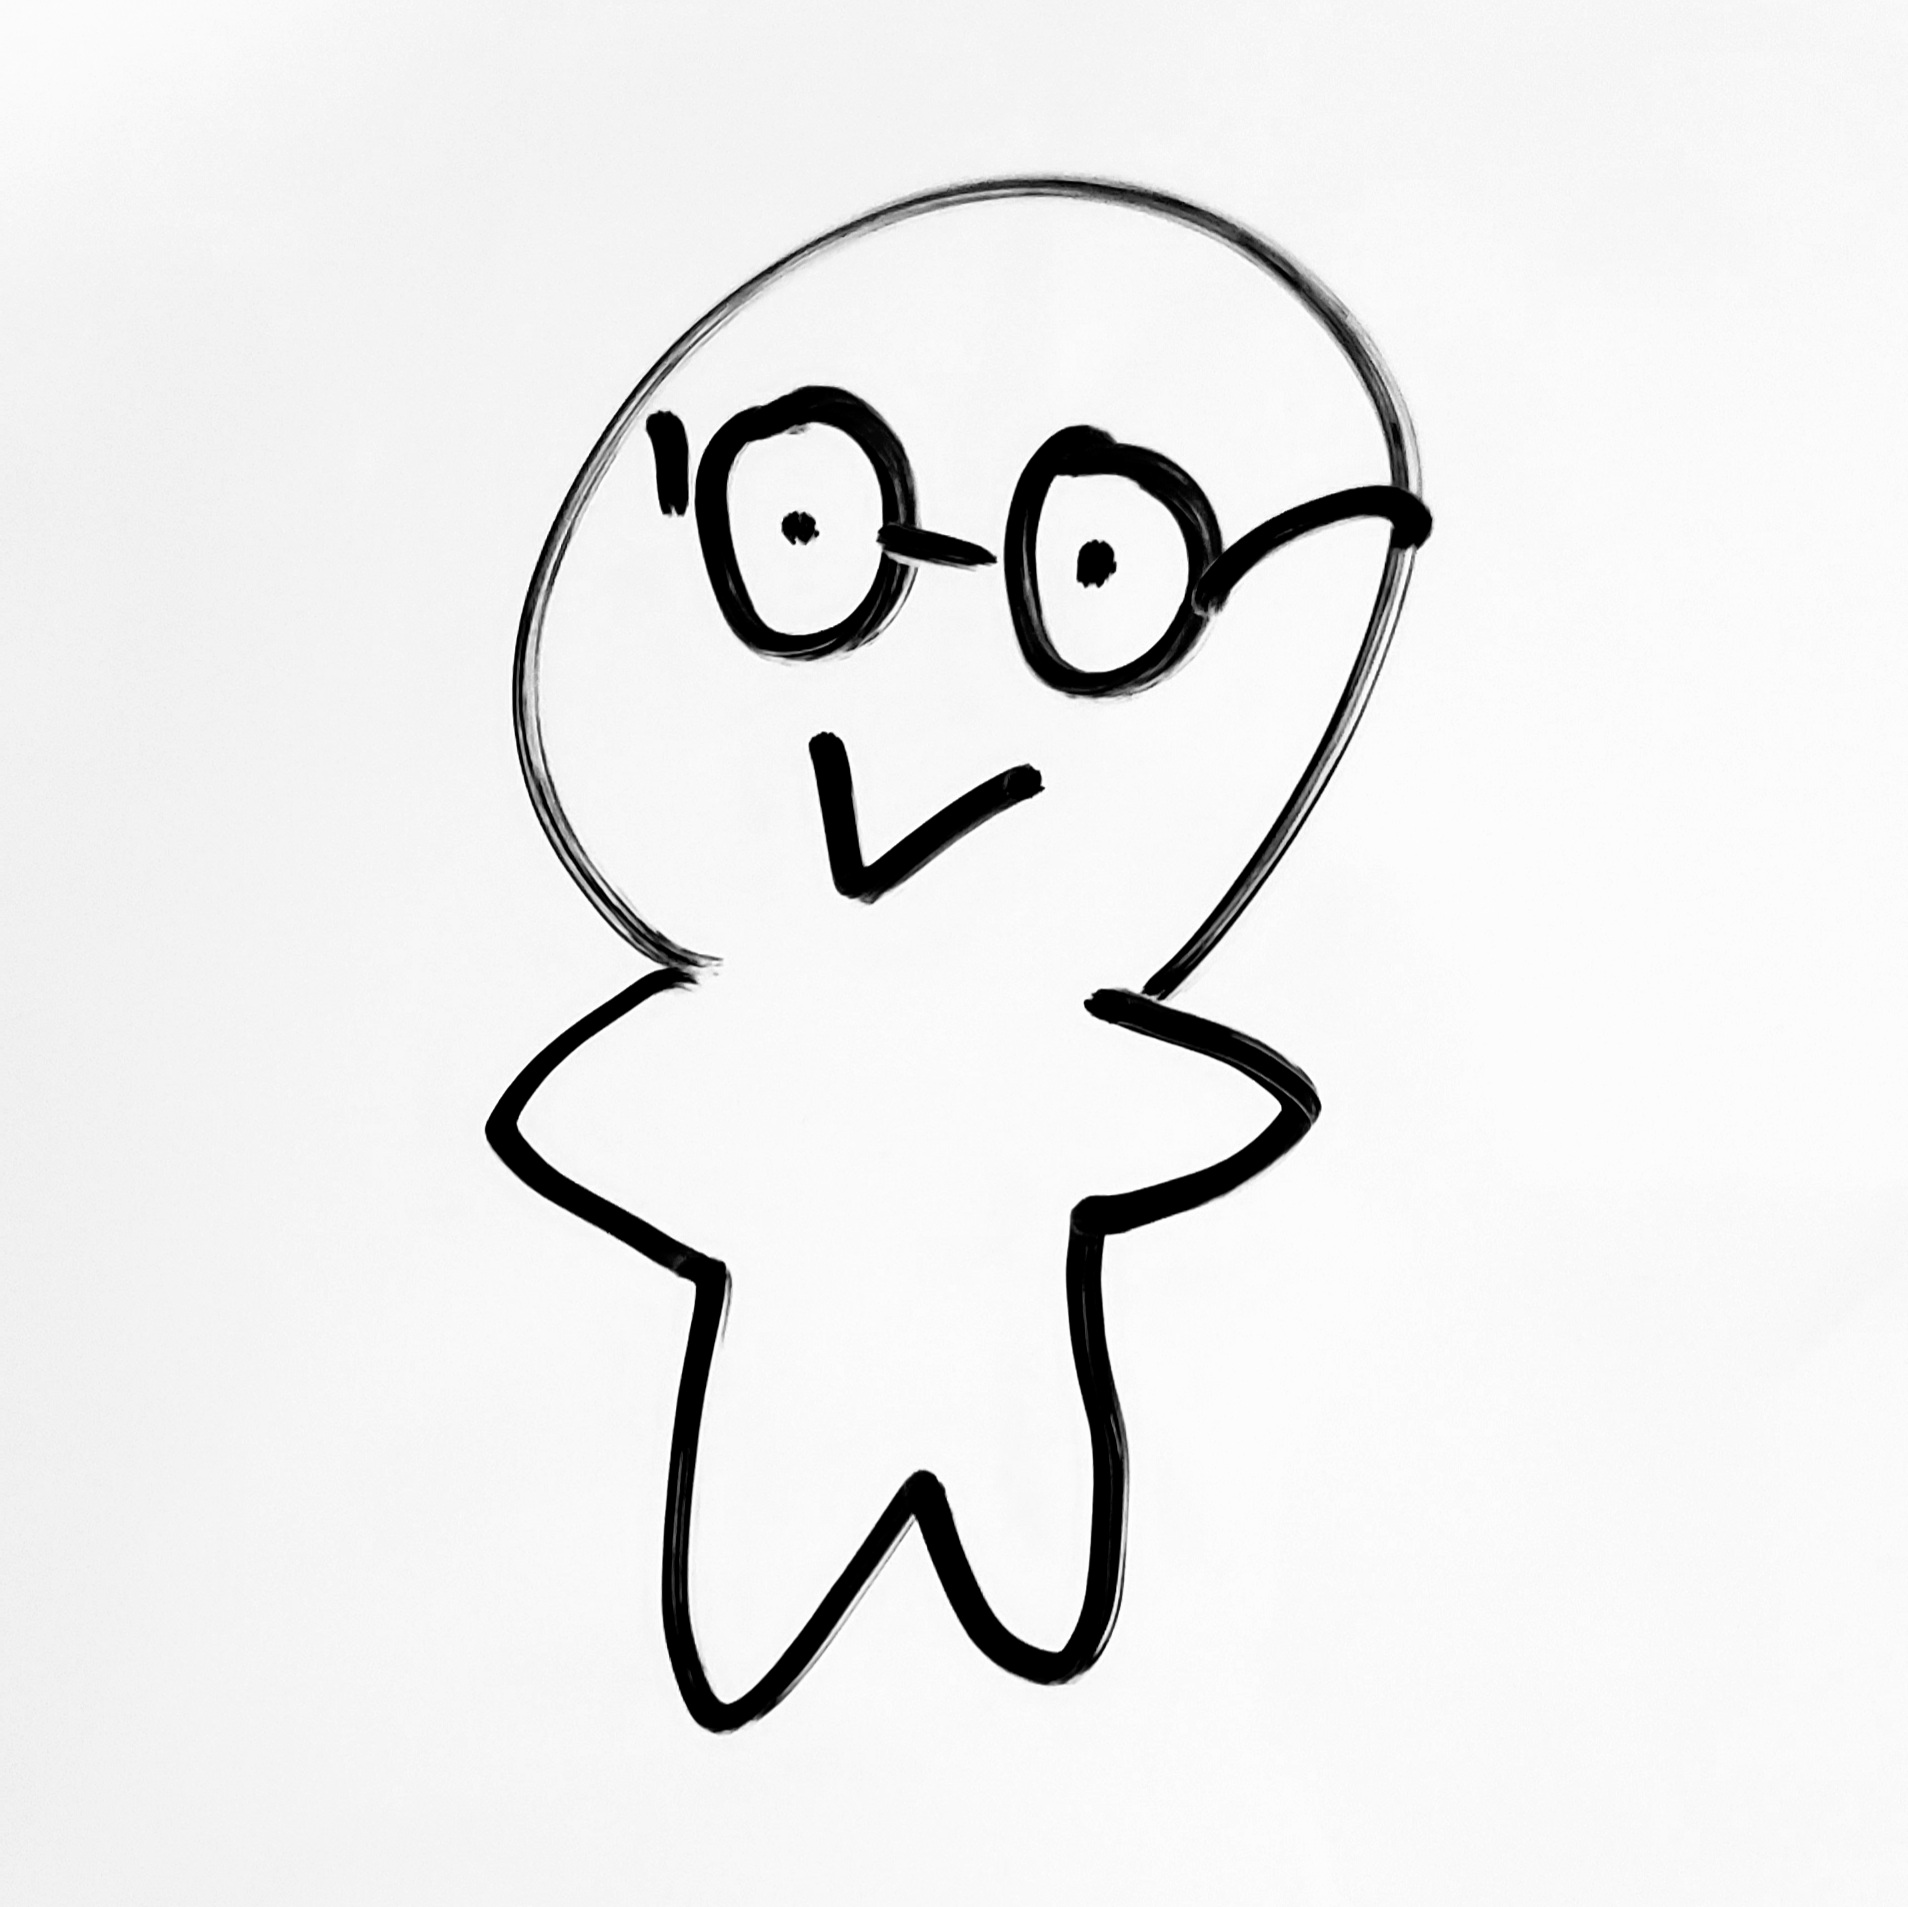
\includegraphics[height=.3\textheight]{figs/fig.jpg}}
    &
    \raisebox{-.5\height}{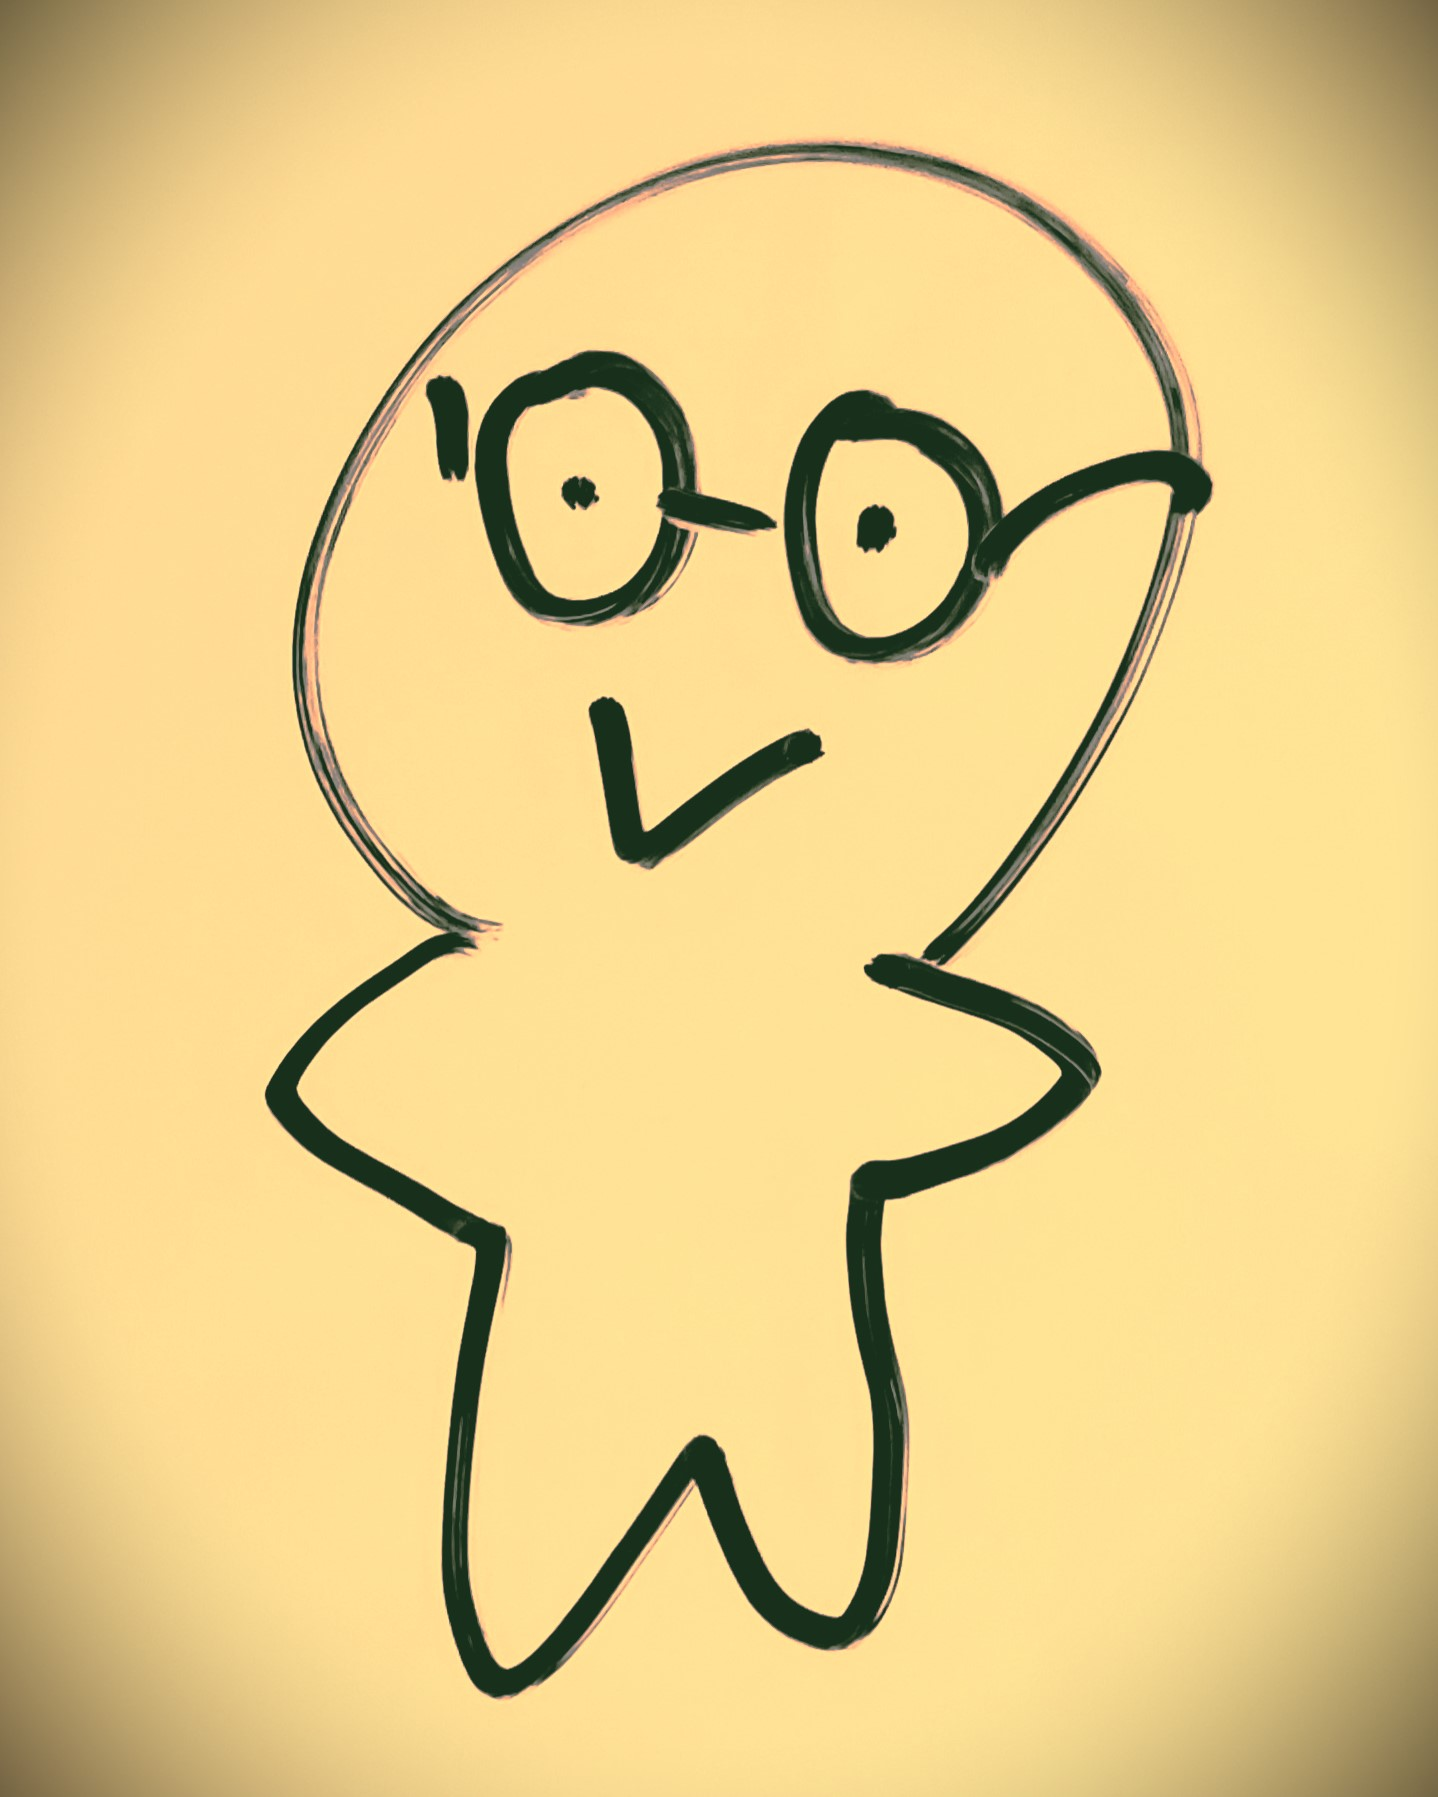
\includegraphics[height=.3\textheight]{figs/fig_mod.jpg}}
    &
    \makecell{makecellを使うと \\ セル内で改行もできる}
\end{tabular}
\end{block}
\end{minipage}
\end{center}

*\verb+\raisebox{-.5\height}{\includegraphics[height=...}+としてある.

\centering
{\footnotesize [参考] \url{https://latex.org/forum/viewtopic.php?t=21730}}
\end{frame}

% \appendix以降はページ番号カウントされない.
\appendix
% \section{付録資料} などと書くとエラーが出るみたい.

\begin{frame}
\frametitle{付録:appendixnumberbeamerパッケージが便利}
\begin{itemize}
    \item このパッケージを使うと,\backslash appendix以降のページを除いてページ番号を計算してくれる.
    \item 実際,これ以降のページにはページ番号が振られていない.
    \item 本体のスライドが5枚,付録が50枚,みたいな状況(?)で,最初のページに1/55と書いてあったら,聴衆はしょんぼりしてしまう.
    \item[*] これは発表者にとっても嬉しくないよね.
\end{itemize}
\end{frame}

\begin{frame}[containsverbatim]
\frametitle{付録:小技集}
$\blacksquare$ 数式モードのblacksquareを使うと見出しっぽくなる
\begin{itemize}
    \item 何も考えずにスライドをつくりたいとき,itemize環境に列記するだけで少し見た目が良くなる.
    \item frameのタイトルはframetitleコマンドを使って指定するようにしている,
    \begin{itemize}
        \item \backslash begin\{frame\}\{タイトル\}でも記述できるが,frameにオプションを渡したいときに挙動がよくわからない.
        \item 例えばラベルをつけようとすると,ビルドできなくなる(と思う).
    \end{itemize}
\end{itemize}

$\blacksquare$ \verb+#特殊記号@を\verbなど+で出力したい場合
\begin{itemize}
    \item デフォルトでは,beamer内でverb / verbatimを使うことができない.
    \item frameのオプションに[containsverbatim]を渡すことで使えるようになる.
\end{itemize}

\begin{block}{}
\begin{description}[ラベルの長さ]
    \item[ラベル] description環境も便利である.
    \item[ラベルの長さ] 一番長いラベルを環境のオプションとして渡すだけで,ラベル幅を調整できる.
    \item[{$x \in [0, 1]$}] こういう風に文字の説明に使うこともできる.
    \item[注意点] ラベル部分に[](角括弧)を使うときは,\{ \dots \}で囲う必要がある.
\end{description}
\end{block}
\end{frame}

% reference, if any
\begin{comment}
\begin{frame}{References}
    % if you have .bib file:
    %\bibliographystyle{unsrt}
    %\bibliography{refs.bib}

    % otherwise:
    \begin{thebibliography}{9}
        \bibitem{aaa}
        \bibitem{bbb}
    \end{thebibliography}
\end{frame}
\end{comment}

\end{document}

